%!TEX program = xelatex

\documentclass[compress]{beamer}
%--------------------------------------------------------------------------
% Common packages
%--------------------------------------------------------------------------
\usepackage[english]{babel}
\usepackage{pgfpages} % required for notes on second screen
\usepackage{graphicx}

\usepackage{multicol}

\usepackage{tabularx,ragged2e}
\usepackage{booktabs}

% fancy source code
% !! require calling latex with -shell-escape !!
\usepackage[cache]{minted}
\renewcommand{\theFancyVerbLine}{
  \sffamily\textcolor[rgb]{0.5,0.5,0.5}{\scriptsize\arabic{FancyVerbLine}}}

\newminted{python}{frame=lines,
                    linenos=true,
                    gobble=4,
                    fontsize=\scriptsize,
                    xleftmargin=1.8em}



%--------------------------------------------------------------------------
% Load theme
%--------------------------------------------------------------------------
\usetheme{hri}

\usepackage{dtklogos} % must be loaded after theme
\usepackage{tikz}
\usetikzlibrary{mindmap,backgrounds,positioning}

\graphicspath{{figs/}}

%--------------------------------------------------------------------------
% General presentation settings
%--------------------------------------------------------------------------
\title{MORSE \& HRI}
\subtitle{Recent Perspectives}
\date{\today}
\author{Séverin Lemaignan, Marc Hanheide, \\ Michael Karg, Harmish Khambhaita,
\\Lars Kunze, \underline{Florian Lier}, \\Ingo Lütkebohle and Grégoire Milliez}

%--------------------------------------------------------------------------
% Notes settings
%--------------------------------------------------------------------------
%\setbeameroption{show notes on second screen}

\begin{document}
%--------------------------------------------------------------------------
% Titlepage
%--------------------------------------------------------------------------

\maketitle

%\begin{frame}[plain]
%	\titlepage
%\end{frame}

%--------------------------------------------------------------------------
% Table of contents
%--------------------------------------------------------------------------
\section*{Overview}
\begin{frame}{Overview}
	% hideallsubsections ist empfehlenswert für längere Präsentationen
	\tableofcontents[hideallsubsections]
\end{frame}

%--------------------------------------------------------------------------
% Content
%--------------------------------------------------------------------------
\section{Brief Recap of MORSE}


\begin{frame}

\begin{figure}
\centering
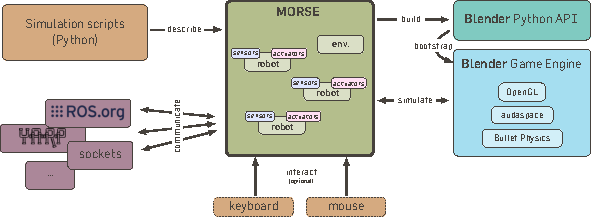
\includegraphics[width=\linewidth]{morse}
%\resizebox{\paperwidth}{!}{%


    %\tikzset{robot/.style={draw, font=\scriptsize, fill opacity=0.5, text opacity=1, fill=white!50}}

    %\begin{tikzpicture}[
    %    >=latex,
    %    every edge/.style={draw, very thick},
    %    cmpt/.style={draw, rounded corners, align=center, inner sep=5pt, fill=black!20},
    %    label/.style={midway, align=center, font=\scriptsize, fill=white}]

    %    \node at (0,0)[cmpt, ultra thick, fill=hriSec2Dark!50] (morsebox) {%
    %        \begin{tikzpicture}
    %            \node (morse) {MORSE};
    %            \node [robot, below=0.2 of morse] (world-update) {Sensors fusion};
    %            \node [robot, below=0.2 of world-update] (geom-model) {Geometric model of the environment};
    %            \node [robot, below=0.2 of geom-model] (fact-prod) {Symbolic facts production};
    %        \end{tikzpicture}
    %    };
    %    \node at (-4, -2.5)[cmpt, fill=hriSec1!50] (ros) {
\includegraphics[height=1cm]{logo-ros}};
    %    \node at (-4.5, -3.5)[cmpt, fill=hriSec1!50] (yarp) {
\includegraphics[height=1cm]{logo-yarp}};
    %    \node at (-3.5, -4.5)[cmpt, fill=hriSec1!50] (socket) {sockets};
    %    \node at (-4.5, -5.5)[cmpt, fill=hriSec1!50] (other_mw) {...};

    %%% SPARK
    %\node at (4,-3.5)[cmpt, fill=hriSec3!50] (spark) {%
    %    \begin{tikzpicture}
    %        \node at (0,0) (geom) {{\sc Spark} -- Geometric \& Temporal Reasoning};
    %        \node [robot, below=0.2 of geom.south west, anchor=north west] (world-update) {Sensors fusion};
    %        \node [robot, right=0.2 of world-update] (geom-model) {Geometric model of the environment};
    %        \node [robot, right=0.2 of geom-model] (fact-prod) {Symbolic facts production};
    %    \end{tikzpicture}
    %    };

    %%%% MHP
    %    \node at (9,0)[cmpt, fill=hriSec3CompDark!50] (mhp) {{\sc mhp} -- Human-aware \\ Motion and Manipulation \\ Planning};

    %%%% SHARY
    %\node at (4,4.5)[cmpt, fill=hriSec1Comp!50] (shary) {%
    %    \begin{tikzpicture}
    %        \node at (0,0) (exec) {Execution Controller};
    %        \node [robot, below=0.2 of exec.south west, anchor=north west] (plans) {Goal \& Plans \\ management};
    %        \node [robot, right=0.2 of plans] (sit-asses) {Situation assessment \\ and context management};
    %        \node [robot, right=0.2 of sit-asses] {Action instantiation, \\ execution and monitoring};
    %    \end{tikzpicture}
    %    };


    %%%% LOWLEVEL
    %\node [cmpt, below=0.7 of spark] (lowlevel) {%
    %    \begin{tikzpicture}
    %        \node at (0,0) (sensori) {Sensorimotor layer};
    %        %\node [subpart, below=0.2 of sensori.south west, anchor=north west, align=left] (perception) {{\bf Perception} \\ 2D markers, RGB-D, motion capture};
    %        %\node [subpart, align=right, right=0.2 of perception] {{\bf Actuation} \\ Head's pan-tilt unit, grippers, arms, wheels};
    %    \end{tikzpicture}
    %};

    %%%% Separation between deliberative layer and sensori-motor layer
    %\draw[dotted, thick] (-8,-5) -- (12, -5);

    %%%% Relations between components
    %\path (shary.340) edge [<->, bend left] node[label] {motion plan \\ requests} (mhp);
    %\path (shary.west) edge [<->, bend right] node[label] {shared \\ plans} (ros);
    %\path (ros) edge [<->, bend right] node[label] {world model and \\ agents beliefs} (morse.170);
    %\path (dialogs) edge [<->, bend left] node[label] {natural language \\ grounding} (morse.190);
    %\path (spark.100) edge [->, bend right] node[label] {symbolic \\ facts} (morse);
    %\path (spark.5) edge [->, bend right] node[label] {environment\\model} (mhp);
    %\path (shary) edge [<->, bend left] node[label] {events, \\ world model and \\ agents beliefs} (morse);
    %\path (shary) edge [<->, bend left] node[label] {action monitoring \\ and management of \\ position hypotheses} (spark);
    %\path (lowlevel) edge [->] (spark);
    %\path (lowlevel.east) edge [<-, bend right=80, looseness=1.5] node[label] {atomic\\actions} (shary.east);

    %\end{tikzpicture}
%}
\end{figure}

\end{frame}

\begin{frame}[fragile]
    \begin{multicols}{2}
        \null \vfill
\begin{pythoncode}
    from random import uniform
    from morse.builder import *
    
    robot = PR2()
    
    for h in range(30):
        human = Human()
        human.translate(
                uniform(-5, 5), 
                uniform(-5, 5), 
                0)

        human.rotate(
                0, 
                0, 
                uniform(0, 360))
    
    env = Environment('sandbox')
\end{pythoncode}

        \vfill \null
        \columnbreak
        \null \vfill
        \begin{figure}
            \centering
            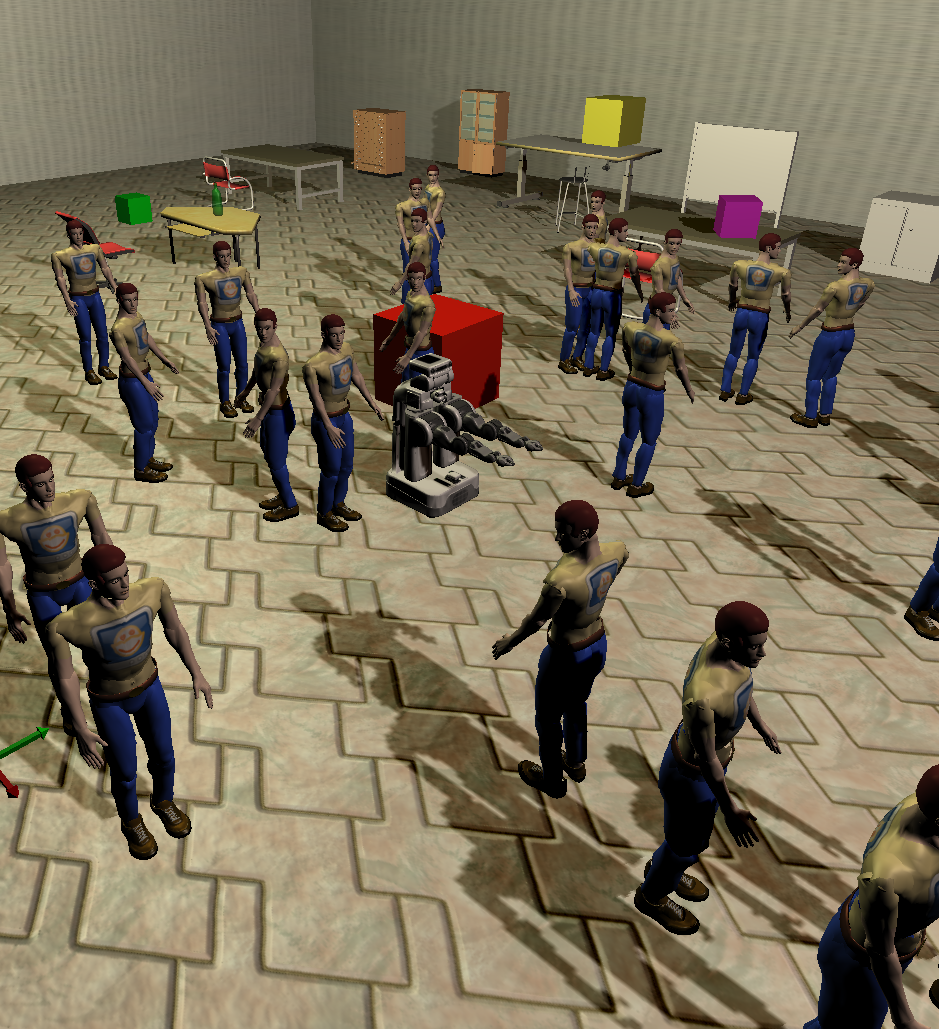
\includegraphics[width=\linewidth]{30humans}
        \end{figure}
        \vfill \null
    \end{multicols}
\end{frame}

\imageframe[Not there yet...]{morse-hri}

\section{Simulating HRI}

\begin{frame}{Situation Assessment with Human}
    \begin{figure}
        \centering
        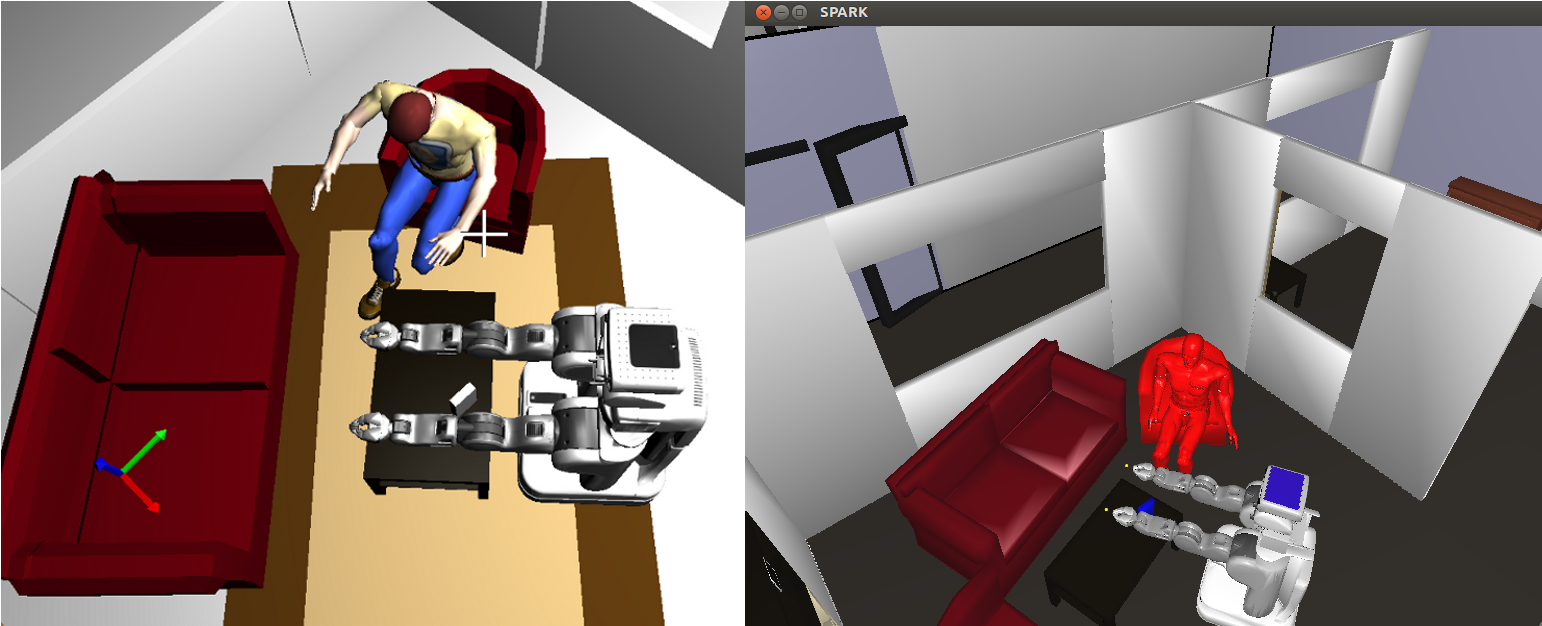
\includegraphics[width=\linewidth]{morsespark}
    \end{figure}

\end{frame}

\begin{frame}{Large Scenarii}
    \begin{figure}
        \centering
        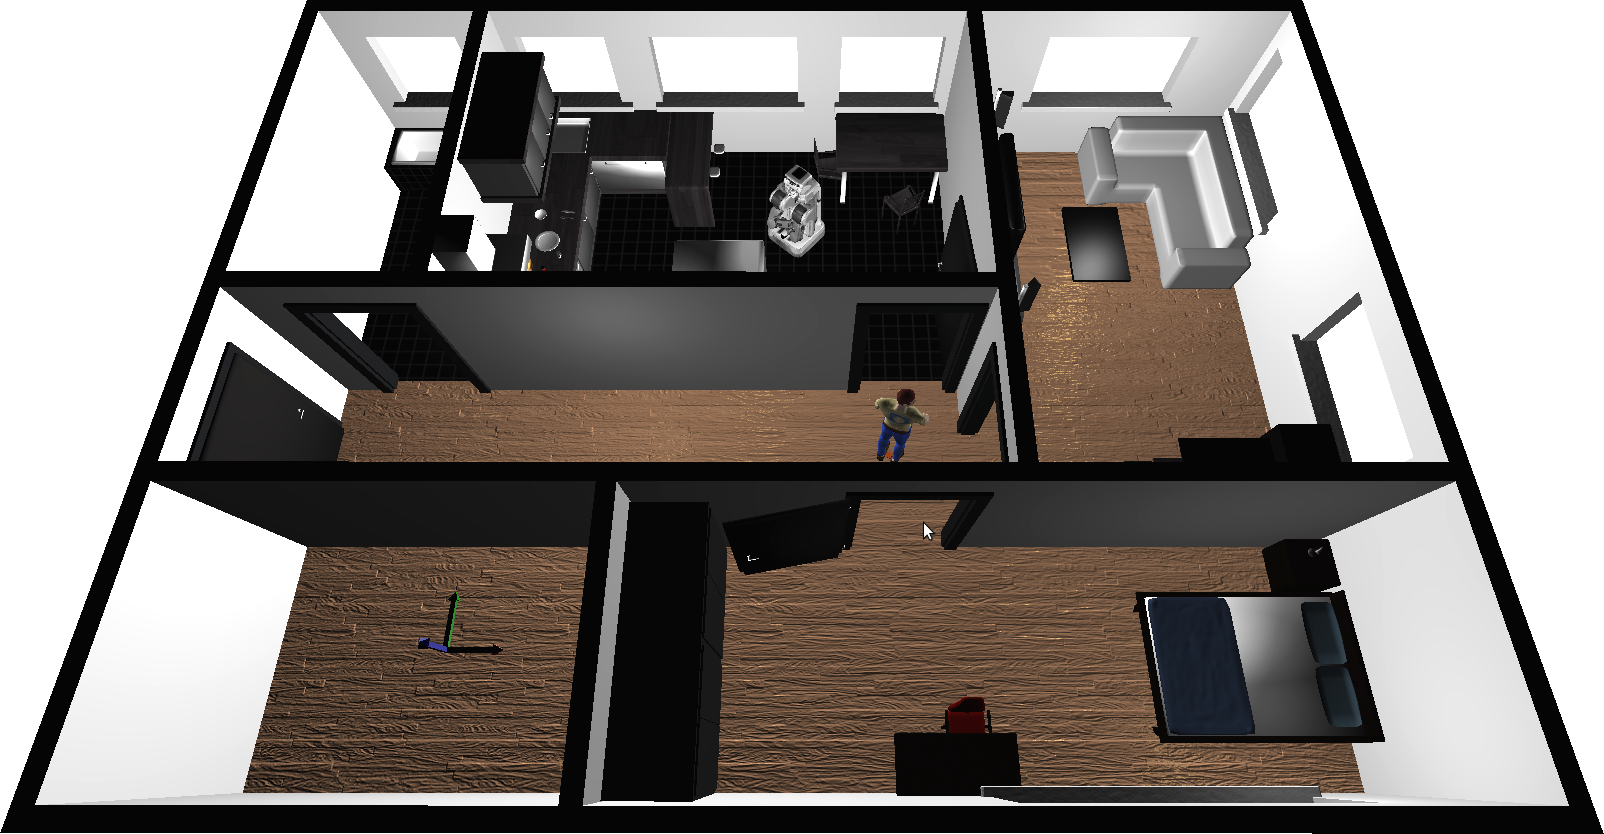
\includegraphics[width=\linewidth]{morse_apartment}
    \end{figure}

\end{frame}

\begin{frame}{Refining Algorithms}
    \begin{figure}
        \centering
        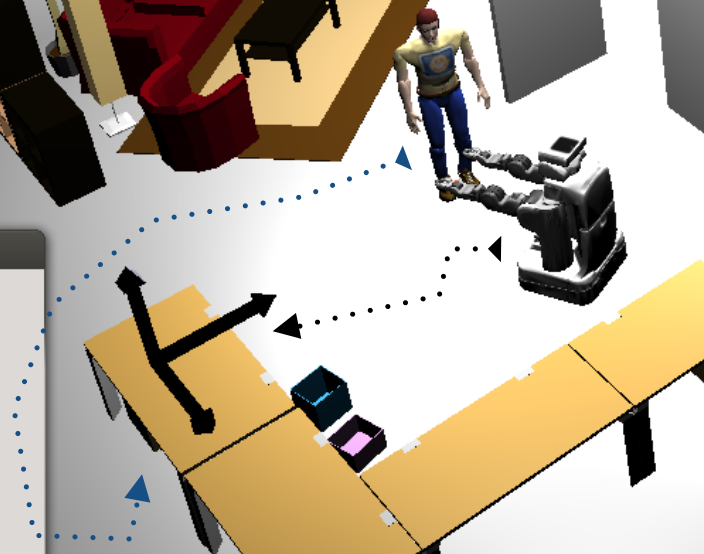
\includegraphics[width=0.8\linewidth]{proto-setup}
    \end{figure}

\end{frame}



\end{document}






